\begin{verbatim}
\subsection{Sine functions}
For given $x \in [0, 2\pi]$ with step size $\pi/12$, we can obtain the evaluations
of \eqref{eq:sine} at $x$ (see Table \ref{tab:sine}), and the corresponding plot
(see Figure \ref{fig:sine}).

\begin{equation}
  \label{eq:sine}
  \begin{cases}
    y_1 = \sin(x/2) \\
    y_2 = \sin(x)   \\
    y_3 = \sin(2x)
  \end{cases}
\end{equation}
\begin{table}[!hbtp]
\centering
\caption{Sine functions}
\label{tab:sine}
\begin{tabular}{ccrr}
\toprule
        $x$ & $\sin(x/2)$ &   $\sin(x)$ &  $\sin(2x)$ \\
\midrule
$0$      & $0$          & $0$  & $0$ \\
$\pi/2$  & $\sqrt{2}/2$ & $1$  & $0$ \\
$\pi$    & $1$          & $0$  & $0$ \\
$3\pi/2$ & $\sqrt{2}/2$ & $-1$ & $0$ \\
$2\pi$   & $0$          & $0$  & $0$ \\
\bottomrule
\end{tabular}
\end{table}
\begin{figure}[!hbtp]
  \centering
  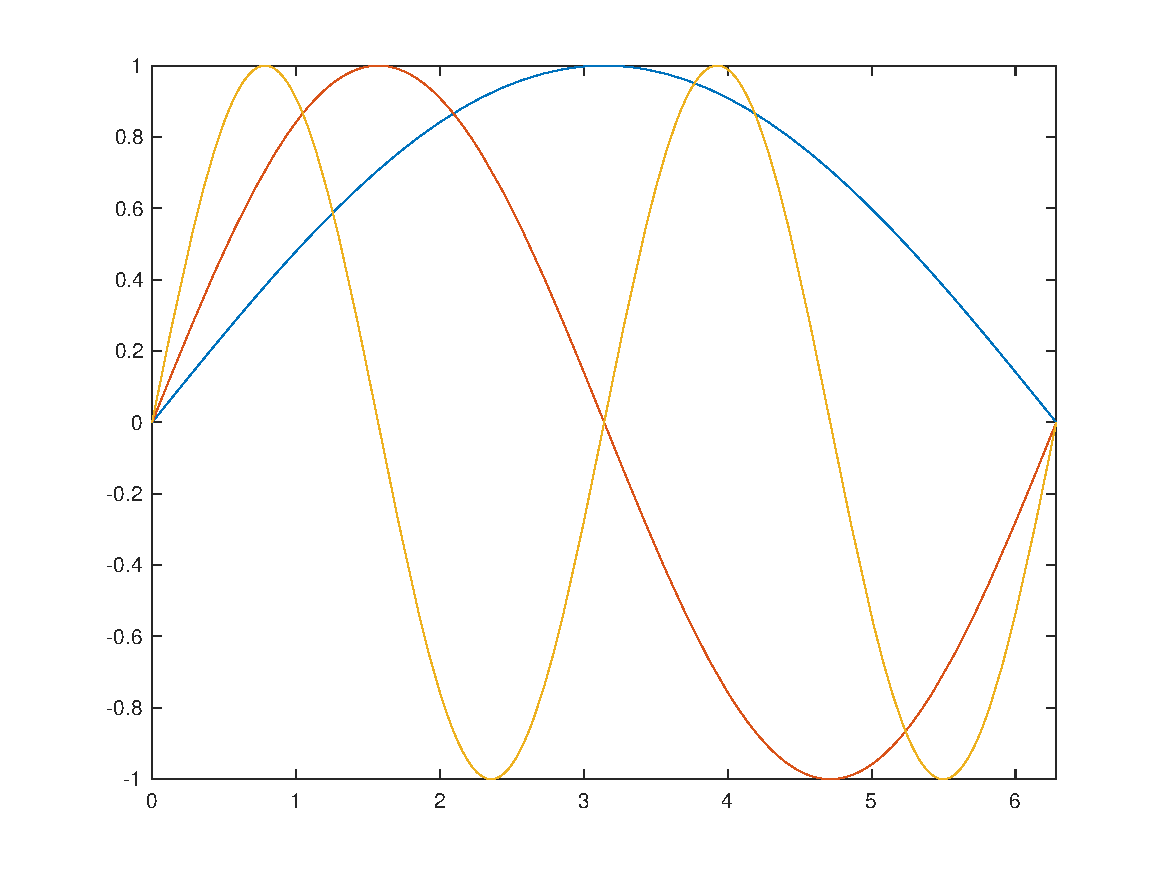
\includegraphics[width=0.3\textheight]{./fig/sine.pdf}
  \caption{Sine functions}
  \label{fig:sine}
\end{figure}

\subsection{Goldbach's Conjecture}
Pursuing this type of analysis more carefully, Hardy and Littlewood in 1923 conjectured
(as part of their famous \textsl{Hardy–Littlewood prime tuple conjecture}) that for any
fixed $c \geq 2$, the number of representations of a large integer $n$ as the sum of $c$
primes $n = p_1 + \cdots + p_{c}$ with $p_1 \leq \cdots \leq p_c$ should be asymptotically
equal to
\begin{equation}
    \label{eq:hardy}
    \left( \prod_{p} \frac{p \gamma_{c,p} (n)}{(p - 1)^c}\right)
    \int_{2 \leq x_1 \leq \cdots \leq x_c: x_1 + \cdots + x_c = n}
    \frac{d x_1 \cdots d x_{c - 1}}{\ln{x_1} \cdots \ln{x_c}},
\end{equation}
where the product is over all primes $p$, and $\gamma_{c, p}(n)$ is the number of
solutions to the equation $n = q_1 + \cdots + q_c \mod p$ in modular arithmetic,
subject to the constraints $q_1, \ldots, q_c \ne 0 \mod p$. This formula
\eqref{eq:hardy} has been rigorously proven to be asymptotically valid for
$c \geq 3$ from the work of Vinogradov, but is till only a conjecture when $c = 2$.
In the latter case, the above formula simplifies to $0$ when $n$ is odd, and to
$$
2 \Pi_2 \left( \prod_{p|n; p \geq 3} \frac{p - 1}{p - 2} \right)
\int_{2}^{n} \frac{dx}{(\ln{x})^2} \approx 2 \Pi_2
\left( \prod_{p|n; p \geq 3} \frac{p - 1}{p - 2} \right) \frac{n}{(\ln{n})^2},
$$
when $n$ is even, where $\Pi_2$ is Hardy-Littlewood's twin prime constant
$$
\Pi_2 := \prod_{p \geq 3} \left( 1 - \frac{1}{(p - 1)^2} \right) = 0.6601618158\ldots
$$
This sometimes known as the \textsf{extended Goldbach conjecture}.

\emph{Reference}: \href{https://en.wikipedia.org/wiki/Goldbach's_conjecture}{Goldbach's conjecture}.
\end{verbatim}
